\documentclass[reprint,amsmath,amssymb.aps]{revtex4-2}


\usepackage{graphicx}
\usepackage{amsmath,amssymb,amsfonts}
\usepackage{dcolumn}
\usepackage{bm}
\usepackage{siunitx}
\sisetup{separate-uncertainty=true}
\usepackage{cleveref}




\begin{document}
\title{Testing Newton's second law in an accelerating system}
\author{Miguel Arenas}
\email{Author for correspondence: 426marenas@frhsd.com}
\author{Callie Butash}
\author{Jake Chin}
\author{Kriti Malhotra}
\author{Grace Nealon}
\author{Petra Rofman}
\affiliation{Science \& Engineering Magnet Program, Manalapan High School, Englishtown, NJ 07726 USA}
\date{\today}

\begin{abstract}
Newton’s Second Law claims that force is the product of mass and acceleration ($\sum F = ma$). It is applied when calculating the acceleration and velocity of a system with limited data. Using a cart and pulley system, we examined the relationships between force, mass, and acceleration. We concluded that the relationship between force and acceleration is directly proportional, while the relationship between mass and acceleration is inversely proportional, confirming Newton’s second law. 
\end{abstract}

\maketitle

\section{Introduction}
Force is the product of mass and acceleration:
\begin{equation}
\sum F = ma,
\label{eq:1}
\end{equation}
where $\sum F$ is the sum of the external forces acting on the system in \unit{\newton}, $m$ is the mass in \unit{\kilo\gram}, and $a$ is the acceleration in \unit{\meter\per\second\squared}. \Cref{eq:1} illustrates how a system's forces depend on the object's mass and acceleration.              

This relationship between force, mass, and acceleration is useful in determining the acceleration that acts on an object without access to information that can be used to calculate acceleration using kinematics equations (eqs~\ref{eq:2}, \ref{eq:3}, and \ref{eq:4}) like initial ($v_0$) and final velocity ($v_f$) measured in \unit{\meter\per\second}, time ($t$) measured in \unit{\second}, and initial ($x_0$) and final position ($x_f$) measured in \unit{\meter}.     
\begin{align}
x_f &= x_0 + v_0 t + \dfrac{1}{2} a t^2 \label{eq:2}\\
v_f &= v_0 + a t \label{eq:3}\\
v_f^2 &= v_0^2 + 2 a (x_f - x_0) \label{eq:4}
\end{align}

To facilitate hypotheses, we set up a system with a cart on a track attached by a string and pulley to a hanging mass (depicted in \cref{fig:1}), allowing force and mass to be varied somewhat independently since some of the mass in the system was subject to gravitational force, while some were not.

We considered the acceleration, force, and mass, and hypothesized that there could be no acceleration in the system. Newton’s first law gives us the static case where 
\begin{equation}
H_0: \sum F = 0.
\label{eq:5}
\end{equation}
Alternatively, we hypothesized that the net force would increase as the mass increased and that the acceleration of the system would decrease as mass increased, therefore the force would increase as the acceleration increased, while acceleration and mass have an inverse relationship \cref{eq:6n2l}:
\begin{equation}
H_1: \sum F = m a.
\label{eq:6n2l}
\end{equation}
Or, we hypothesized that either Newton’s laws wouldn’t apply, or something was erroneous with the considered forces, resulting in the force being equal to un-modeled forces acting that have a significant effect on acceleration (\cref{eq:7} and \cref{eq:8}).
\begin{align}
H_2: \sum F &\neq 0, \label{eq:7}\\
H_3: \sum F &\neq ma. \label{eq:8} 
\end{align}
These hypotheses were tested through a total of six trials, with a cart that had a constant weight, and different masses on the other end of the pulley. The time was measured to calculate the relationships between force, mass, and acceleration for both values of hanging mass. 













\section{Methods and materials}

\subsection{Tests}
\begin{figure}
\begin{center}
\includegraphics[width=\columnwidth]{fig1.png}
\end{center}
\caption{Track, cart, and pulley system used for experiments. Total track length 1.0m.}
\label{fig:1}
\end{figure}
Tests ($n=6$) were conducted using a track, cart, and pulley system (\cref{fig:1}). The system included a \qty{1.0}{\meter} aluminum test track (Pasco Scientific; Roseville, CA) clamped to a table. The system was outfitted with a wheeled cart (Pasco Scientific; Roseville, CA) with ball bearings and knife-edge wheels. The cart's mass was \qty{0.493}{\kilo\gram} and it carried a \qty{1.000}{\kilo\gram} mass for a total mass of \qty{1.493}{\kilo\gram}. Attached to the cart was a string that looped over a pulley clamped to the table. On the other side of the string, for the first three trials, was a \qty{0.050}{\kilo\gram} mass, which was swapped out for a \qty{0.200}{\kilo\gram} mass for the last three trials. The hanging masses provided gravitational force to drive the system. The cart was released from rest and allowed to accelerate. We measured the time it took for the cart to move from rest \qty{0.70}{\meter} along the track. Data were logged in a Google Document (Google; Mountain View, CA) on a school-issued Google Chromebook (Google; Mountain View, CA). 

\subsection{Acceleration calculations}
\begin{figure}
\begin{center}
\includegraphics[width=\columnwidth]{fig2.png}
\end{center}
\caption{Free body diagrams for $m_1$ (left) and $m_2$ (right) created in Google Drawings.}
\label{fig:2}
\end{figure}

The expected acceleration can be calculated using the tensions of each mass. As seen in \cref{fig:2}, the mass on the track moving horizontally is $m_1$ and the mass falling is $m_2$. The track is frictionless, so the force acting on $m_1$ equals the tension and is calculated as
\begin{equation}
F_1 = m_1 a = T.
\label{eq:9}
\end{equation}
The tension is also acting upward on $m_2$, yielding
\begin{equation}
F_2 = -m_2 a = T - m_2 g.
\label{eq:10}
\end{equation}
Combining \cref{eq:9} and \cref{eq:10} and manipulating gives the system acceleration $a$ as a function of gravitational acceleration $g$ and the known masses $m_1$ and $m_2$:
\begin{equation}
a = \dfrac{m_2}{m_1 + m_2} g.
\label{eq:11}
\end{equation}

The measured time data were also used to calculate acceleration via kinematics assuming uniform motion \cite{tipler}:
\begin{equation}
x = x_0 + v_0 t + \dfrac{1}{2} a t^2.
\label{eq:12}
\end{equation}
Selecting $x_0=0$ and recognizing $v_0=0$, \cref{eq:12} can be solved for acceleration:
\begin{equation}
a = \dfrac{2 x}{t^2},
\label{eq:13}
\end{equation}
where $x=\qty{0.70}{\meter}$ is the length of the track, and $t$ is measured during each trial. 







\section{Results}
Tables~\ref{tab:1} and \ref{tab:2} display the time data we collected for calculating the acceleration. \Cref{fig:3} shows calculated acceleration for all trials. 

\begin{table}
\caption{Data from experiments when the cart was \qty{1.000}{\kilo\gram} and the pulley was \qty{0.050}{\kilo\gram}.} 
\label{tab:1}
\begin{center}
\begin{tabular}{ll}
trial & time (\unit{\second}) \\
1 & 2.43\\
2 & 2.22\\
3 & 2.28
\end{tabular}
\end{center}
\end{table}
	
\begin{table}
\caption{Data from experiments when the cart was \qty{1.000}{\kilo\gram} and the pulley was \qty{0.200}{\kilo\gram}.}
\label{tab:2}
\begin{center}
\begin{tabular}{ll}
trial & time (\unit{\second}) \\
1 & 1.19\\
2 & 0.91\\
3 & 0.91
\end{tabular}
\end{center}
\end{table}	


\begin{figure}
\begin{center}
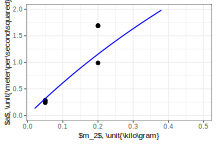
\includegraphics[width=\columnwidth]{fig3.png}
\end{center}
\caption{The calculated acceleration of the three trials for each pulley. This includes the \qty{0.050}{\kilo\gram} mass and the \qty{0.200}{\kilo\gram} mass. The results are limited to two hanging values (\qty{0.050}{\kilo\gram} and \qty{0.200}{\kilo\gram}). Future experiments could include more variation in between to strengthen the observed trends further.}
\label{fig:3}
\end{figure}






\section{Discussion}
%As seen from Tables 1 and 2 and Figure 3, the trials with the 0.050 kg mass have a lower acceleration than the trials with the 0.200 kg mass.
%        The data proves our hypothesis of an inverse relationship between mass and acceleration and a direct relationship between force and acceleration.

\subsection{Can we confirm that $\sum F=ma$ through experimentation?}
Our trials demonstrated that as the pulley's mass, or the gravitational force, increases, the cart's acceleration increases. This supported our hypothesis $\sum F = ma$ \cref{eq:6n2l}. The force acting on the system increased by increasing the pulley's mass. The experimental data corroborated the hypothesis because the increased pulley mass and acceleration illustrate a direct relationship between force and acceleration. Our data showed a consistent pattern where an increase in the mass of the pulley increased the net force creating an increase in acceleration. This suggests that acceleration and force are proportional, ensuring that mass is constant \cref{eq:6n2l}. 

\subsection{Sources of experimental error}
A potential source of experimental error stems from the movement of the track between trials. This caused slight differences in tension, potentially affecting the calculated acceleration of the cart. Additionally, the person's timing was not consistent across all trials, nor were they rotated methodically by trial. This could result in small inconsistencies with the timing that may skew the results of calculating acceleration using a formula involving time or any other calculations involving time. In further testing, the time can be measured with sensors or videos to be more accurate. Furthermore, the expected acceleration was calculated assuming the string was massless and friction had no effect on the cart. Since the experiment used a string with mass and did not eradicate the force of friction, this could result in possible differences between the experimental and expected acceleration.








\section{Acknowledgments}
We thank several anonymous reviewers who provided thoughtful comments on our manuscript; Sir Issac Newton for the discovery of his three laws of motion; and Antonella Ortega for her momentum writeup as a reference. 

%Contributions 
PR wrote the abstract, introduction, test description, part of the discussion, and recorded data during the trials. MA created graphs of the results and helped describe them and draw conclusions. CB made the free-body diagrams and momentum track diagrams, computed acceleration, and wrote aspects of the discussion and parts of other sections. KM wrote the discussion and part of the results, noted the materials, timed the trials, and recorded the results. JC wrote about the sources of the experimental error and helped collect data and the abstract. GN led the track's setup, wrote out the procedures, and conducted each trial when we collected data. Everyone contributed to editing, proofreading, and assisting others with the sections they worked on.





\bibliographystyle{abbrvnat}
\bibliography{lab.bib}
\end{document}
